% !Mode:: "TeX:UTF-8"%確保文檔utf-8編碼
%新加入的命令如下:addchtoc addsectoc reduline showendnotes hlabel
%新加入的环境如下:common-format  fig linefig xverbatim

\documentclass[11pt,oneside]{book}
\newlength{\textpt}
\setlength{\textpt}{11pt}
\newif\ifphone
\phonefalse


\usepackage{myconfig}
\usepackage{mytitle}



\begin{document}
\frontmatter

\titlea{tikz制图指南}
\titleb{在xelatex指南之上}
\titlec{主要是文档中inline的制图,大型复杂制图还是考虑外部绘图软件。}
\author{万泽}
\authorinfo{作者:湖南常德人氏}
\editor{德山书生}
\email{a358003542@gmail.com}
\editorinfo{编者:德山书生,湖南常德人氏。}
\version{0.01}
\titleLC

\addchtoc{前言}
\chapter*{前言}
\begin{common-format}
TikZ is not an interactive drawing program.

1.Graphics with TikZ Andrew Mertz and William Slough

2.A very minimal introduction to TikZ Jacques Crémer

3.the tikz 官方文档,这个用texdoc命令调不出官方文档,用google搜索“tikz pdf”吧
%这里空一行。

\end{common-format}


\addchtoc{目录}
\setcounter{tocdepth}{2}
\tableofcontents

\begin{common-format}
\mainmatter

\section{准备工作}
tikz宏包的加载是必须的,因为我这里myconfig.sty里面的已经加载了chemfig宏包,而chemfig宏包又加载了tikz宏包,所以不需要修改什么了。


\begin{Verbatim}
\tikz{\draw (1,0) -- (0,1) -- (-1,0) -- (0,-1) -- cycle;}

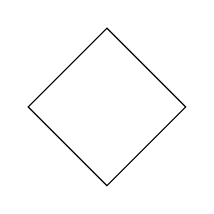
\begin{tikzpicture}
\draw (1,0) -- (0,1) -- (-1,0) -- (0,-1) -- cycle;
\end{tikzpicture}
\end{Verbatim}

\tikz{\draw (1,0) -- (0,1) -- (-1,0) -- (0,-1) -- cycle;}

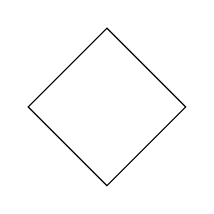
\begin{tikzpicture}
\draw (1,0) -- (0,1) -- (-1,0) -- (0,-1) -- cycle;
\end{tikzpicture}

有两种使用方法,一种命令式的,一种环境式的。命令式用tikz命令包围起来,命令式是inline模式的。环境式用tikzpicture命令包围起来。

这里推荐KTikZ软件,在ubuntu软件中心里面就有,用这个软件可以边写tikz代码边看画的图形,还可以导出图形,早期推荐先使用这个软件练练手熟悉下tikz制图代码。值得一提的是这个软件不支持中文注释,会生成乱码。



\chapter{tikz基础}
\section{第一个例子}
\subsection{画网格}
\begin{Verbatim}

\begin{tikzpicture}
\draw[step=1,color=gray!40] (-2,-2) grid (2,2);
\end{tikzpicture}
\end{Verbatim}


\begin{tikzpicture}
\draw[step=1,color=gray!40] (-2,-2) grid (2,2);
\end{tikzpicture}

step是网格之间的间距,color是网格的颜色。第一个坐标点是网格的左底点,第二个坐标点是网格的右顶点。我们可以看到tikzpicture下每一条命令最后都要跟一个分号\emph{;}。

\subsection{画直线}
\begin{Verbatim}
\begin{tikzpicture}
\draw[step=1,color=gray!40] (-2,-2) grid (2,2);
\draw (-3,0) -- (3,0);
\draw (0,-3) -- (0,3);
\end{tikzpicture}
\end{Verbatim}

\begin{tikzpicture}
\draw[step=1,color=gray!40] (-2,-2) grid (2,2);
\draw (-3,0) -- (3,0);
\draw (0,-3) -- (0,3);
\end{tikzpicture}

画直线就是两个坐标点相连,中间 -{}-{} 符号表示直线的意思。之前网格是grid表示网格的意思。

\subsubsection{直线带上箭头}
draw命令可以跟上可选项\textbf{->},这样直线的右端就有一个箭头了。此外还有:\textbf{->>},\textbf{->|},\textbf{-to},\textbf{-latex},\textbf{-stealth}。

他们的效果从上到下依次演示如下:

\begin{tikzpicture}
\draw[->] (-3,3) -- (3,3);
\draw[->>] (-3,2) -- (3,2);
\draw[->|] (-3,1) -- (3,1);
\draw[-to] (-3,0) -- (3,0);
\draw[-latex] (-3,-1) -- (3,-1);
\draw[-stealth] (-3,-2) -- (3,-2);
\end{tikzpicture}

类似的还有左端比如\textbf{<-},或者两端比如\textbf{latex-latex},这里就不多说了。

\subsection{画圆}
接著上面的图案画一个圆,加入了以下代码:\\
\verb+\draw (0,0) circle (1); +

\begin{tikzpicture}
\draw[step=1,color=gray!40] (-2,-2) grid (2,2);
\draw[->] (-3,0) -- (3,0);
\draw[->] (0,-3) -- (0,3);
\draw (0,0) circle (1); 
\end{tikzpicture}

其中第一个点是圆中心,circle表示画圆,第二个参数是半径大小。


\subsection{画椭圆}
接著画一个椭圆:\\
\verb+\draw (0,0) ellipse (1 and 0.5);+

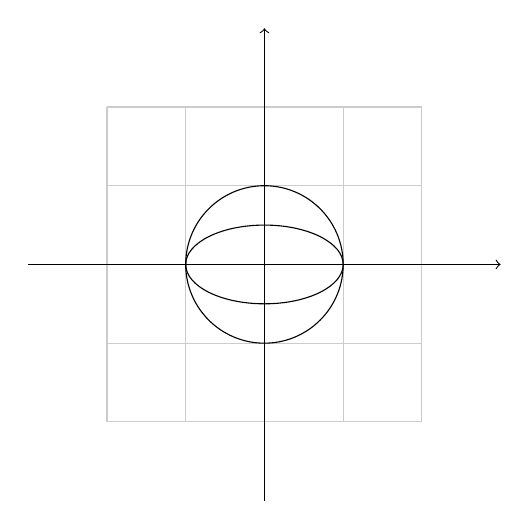
\begin{tikzpicture}
\draw[step=1,color=gray!40] (-2,-2) grid (2,2);
\draw[->] (-3,0) -- (3,0);
\draw[->] (0,-3) -- (0,3);
\draw (0,0) circle (1); %
\draw (0,0) ellipse (1 and 0.5);
\end{tikzpicture}

这里第一个点是椭圆的中心点,ellipse表示画椭圆,后面参数两个值第一个是a也就是椭圆的半长,第二个是b也就是椭圆的半高。

\subsection{点的定义}
tikz中定义一个点方便之后使用:

\begin{Verbatim}
\path (1,1) coordinate (point001);
\path (2,0) coordinate (point002);
\draw[dotted] (point001) -- (point002)  ;
\end{Verbatim}

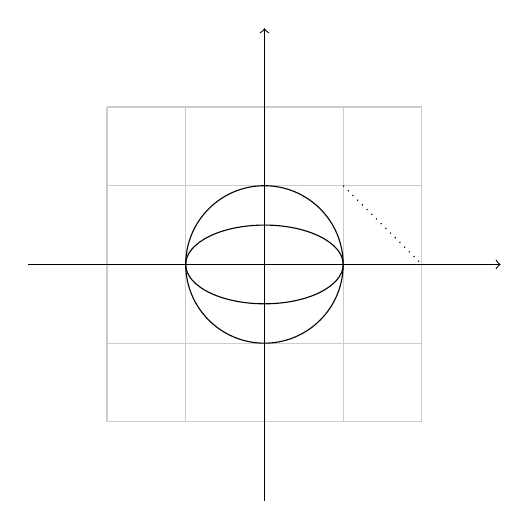
\begin{tikzpicture}
\draw[step=1,color=gray!40] (-2,-2) grid (2,2);
\draw[->] (-3,0) -- (3,0);
\draw[->] (0,-3) -- (0,3);
\draw (0,0) circle (1); %
\draw (0,0) ellipse (1 and 0.5);
\path (1,1) coordinate (point001);
\path (2,0) coordinate (point002);
\draw[dotted] (point001) -- (point002)  ;
\end{tikzpicture}

这里代码的第6,7行定义了两个点,名字叫做point001和point002。然后用这两个点作为参数画了一个直线,这个直线有可选项\textbf{dotted},点线样式。

\subsection{放大图形}
在tikzpicture环境后面跟上可选项[scale=2],即将图形放大两倍。注意控制别越界了。

\begin{tikzpicture}[scale=2]
\draw[step=1,color=gray!40] (-2,-2) grid (2,2);
\draw[->] (-3,0) -- (3,0);
\draw[->] (0,-3) -- (0,3);
\draw (0,0) circle (1); %
\draw (0,0) ellipse (1 and 0.5);
\path (1,1) coordinate (point001);
\path (2,0) coordinate (point002);
\draw[dotted] (point001) -- (point002)  ;
\end{tikzpicture}


\subsection{点的相对偏移}
现在加上这样两行代码:

\begin{Verbatim}
\draw[<->] (0,-2) -- ++(-1,1) -- ++(-1,-1);
\draw[dashed] (0,1) -- +(-1,1) -- +(-2,0);
\end{Verbatim}

\begin{tikzpicture}[scale=2]
\draw[step=1,color=gray!40] (-2,-2) grid (2,2);
\draw[->] (-3,0) -- (3,0);
\draw[->] (0,-3) -- (0,3);
\draw (0,0) circle (1); %
\draw (0,0) ellipse (1 and 0.5);
\path (1,1) coordinate (point001);
\path (2,0) coordinate (point002);
\draw[dotted] (point001) -- (point002)  ;
\draw[latex-latex] (0,-2) -- ++(-1,1) -- ++(-1,-1);
\draw[dashed] (0,1) -- +(-1,1) -- +(-2,0);
\end{tikzpicture}

tikz中有一个重要的概念,当前点,然后点可以通过当前点根据相对偏移来确定一个新的点。上面代码第9行的\textbf{++}符号和第10行的\textbf{+}符号都根据当前点然后进行了$ \Delta x $和$ \Delta y $的相对偏移从而确定了一个新的点。这两个符号的区别在于是不是更新当前点数据。++符号更新当前点,而+符号不更新。


\subsection{画长方形}
现在加上这一行代码来画一个长方形:\\
\verb+\draw[color=red] (-1,-1) rectangle (1,1);+

\begin{tikzpicture}[scale=2]
\draw[step=1,color=gray!40] (-2,-2) grid (2,2);
\draw[->] (-3,0) -- (3,0);
\draw[->] (0,-3) -- (0,3);
\draw (0,0) circle (1); %
\draw (0,0) ellipse (1 and 0.5);
\path (1,1) coordinate (point001);
\path (2,0) coordinate (point002);
\draw[dotted] (point001) -- (point002)  ;
\draw[<->] (0,-2) -- ++(-1,1) -- ++(-1,-1);
\draw[dashed] (0,1) -- +(-1,1) -- +(-2,0);
\draw[color=red] (-1,-1) rectangle (1,1);
\end{tikzpicture}

这里使用了可选项\textbf{color=red}来控制线条的颜色,然后画长方形的第一个点是左底点,rectangle表示画长方形,第二个点表示右顶点。


\subsection{画函数}
画函数的功能是通过外部程序gnuplot来实现了,所以需要打开\verb+--shell-escape+,或者\verb+--enable-write18+

这里最后加了一个语句:\\
\verb+\draw[domain=-pi:pi,color=green] plot function{sin(x)};+

\begin{tikzpicture}[scale=1.8]
\draw[step=1,color=gray!40] (-2,-2) grid (2,2);
\draw[->] (-3,0) -- (3,0);
\draw[->] (0,-3) -- (0,3);
\draw (0,0) circle (1); %
\draw (0,0) ellipse (1 and 0.5);
\path (1,1) coordinate (point001);
\path (2,0) coordinate (point002);
\draw[dotted] (point001) -- (point002)  ;
\draw[<->] (0,-2) -- ++(-1,1) -- ++(-1,-1);
\draw[dashed] (0,1) -- +(-1,1) -- +(-2,0);
\draw[color=red] (-1,-1) rectangle (1,1);
\draw[domain=-pi:pi,color=green] plot function{sin(x)};
\end{tikzpicture}

这里可选项\textbf{domain=-pi:pi}控制画的函数的x范围,可以直接用pi表示π,然后接下来plot function表示画一个函数,接下来的花括号里面放着gnuplot的各种命令,这里就是简单的$ sin(x) $


\chapter{画画的理论讨论}





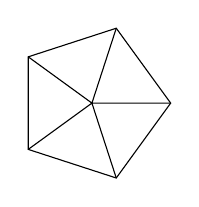
\begin{tikzpicture}
% Define the points of a regular pentagon
\path (0,0) coordinate (origin);
\path (0:1cm) coordinate (P0);
\path (1*72:1cm) coordinate (P1);
\path (2*72:1cm) coordinate (P2);
\path (3*72:1cm) coordinate (P3);
\path (4*72:1cm) coordinate (P4);
% Draw the edges of the pentagon
\draw (P0) -- (P1) -- (P2) -- (P3) -- (P4) -- cycle;
% Add "spokes"
\draw (origin) -- (P0) (origin) -- (P1) (origin) -- (P2)
(origin) -- (P3) (origin) -- (P4);
\end{tikzpicture}

he concept of the current point plays an important role when multiple actions
are involved. For example, suppose two line segments are drawn joining points
P and Q along with Q and R

A relative point may be defined by providing offsets in each of the horizontal
and vertical directions.

%\path (P) ++(∆x,∆y) coordinate (Q);
%Alternately, the offset may be specified with polar coordinates. For example,
%given angle α and radius r, with an appropriate dimensional unit dim, the com-
%mand:
%\path (P) ++(α:rim) coordinate (Q);

There are two forms of relative points — one which updates the current point
and one which does not. The ++ prefix updates the current point while the +
prefix does not.

\begin{tikzpicture}
\draw (0,0) -- ++(1,0) -- ++(1,1) -- ++(1,-1);
\end{tikzpicture}

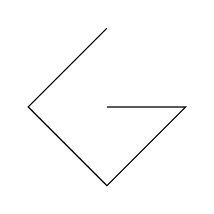
\begin{tikzpicture}
\draw (0,0) -- +(1,0) -- +(0,-1) -- +(-1,0) -- +(0,1);
\end{tikzpicture}

every offset which appears is performed
relative to the initial point, ( 0, 0 ) .

– Grids and rectangles

– Circles and ellipses
– Arcs
– Bézier curves

\begin{tikzpicture}
\draw (0,0) rectangle (1,1)
rectangle (3,2)
rectangle (4,3);
\end{tikzpicture}

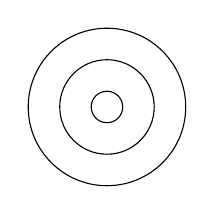
\begin{tikzpicture}
\draw (0,0) circle (1cm)
circle (0.6cm)
circle (0.2cm);
\end{tikzpicture}

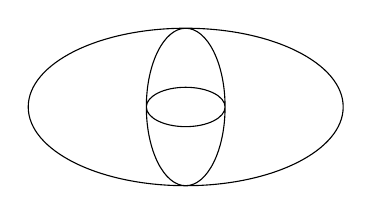
\begin{tikzpicture}
\draw (0,0) ellipse (2cm and 1cm)
ellipse (0.5cm and 1 cm)
ellipse (0.5cm and 0.25cm);
\end{tikzpicture}

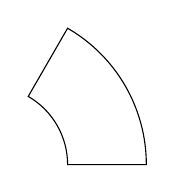
\begin{tikzpicture}
\draw (0:1cm) -- (0:2cm)
arc (0:60:2cm) -- (60:1cm)
arc (60:0:1cm) -- cycle;
\end{tikzpicture}


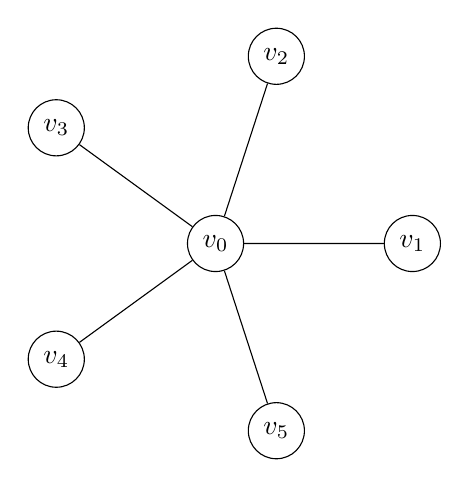
\begin{tikzpicture}[scale=2.5]
\tikzstyle{every node}=[draw,shape=circle];
\path (0:0cm)
node (v0) {$v_0$};
\path (0:1cm)
node (v1) {$v_1$};
\path (72:1cm)
node (v2) {$v_2$};
\path (2*72:1cm) node (v3) {$v_3$};
\path (3*72:1cm) node (v4) {$v_4$};
\path (4*72:1cm) node (v5) {$v_5$};
\draw (v0) -- (v1)
(v0) -- (v2)
(v0) -- (v3)
(v0) -- (v4)
(v0) -- (v5);
\end{tikzpicture}
%这里空一行

\end{common-format}
\end{document}



